% =====================================================================
%  Draf Latar Belakang untuk ditinjau Dosen Pembimbing
%  Kompilasi: pdflatex latar-belakang-dosen.tex (dua kali)
% =====================================================================
\documentclass[11pt,a4paper]{article}

\usepackage[a4paper,margin=2.5cm]{geometry}
\usepackage[T1]{fontenc}
\usepackage[utf8]{inputenc}
\usepackage[scaled=0.95]{helvet}
\renewcommand{\familydefault}{\sfdefault}
\usepackage{microtype}
\setlength{\parindent}{0pt}
\setlength{\parskip}{5pt}
\linespread{1.08}

\usepackage[table]{xcolor}
\usepackage{tabularx}
\usepackage{array}
\usepackage{enumitem}
\usepackage{titlesec}
\usepackage{caption}
\usepackage{float}
\usepackage{pifont}
\usepackage{tikz}
\usetikzlibrary{positioning,arrows.meta}
\usepackage[hidelinks]{hyperref}

\definecolor{hdrgreen}{HTML}{E6EFC5}
\definecolor{subtle}{HTML}{6B7280}
\definecolor{secline}{HTML}{4338CA}
\definecolor{okline}{HTML}{16A34A}
\definecolor{badline}{HTML}{DC2626}
\definecolor{ink}{HTML}{0F172A}

\newcommand{\hdr}[1]{\cellcolor{hdrgreen}\textbf{#1}}
\newcommand{\cmark}{\textcolor{okline}{\ding{51}}}
\newcommand{\xmark}{\textcolor{badline}{\ding{55}}}
\newcommand{\pmark}{\textcolor{subtle}{\ding{108}}}

\titleformat{\section}{\large\bfseries\raggedright}{\thesection.}{0.4em}{}
\titleformat{\subsection}{\normalsize\bfseries\raggedright}{\thesubsection}{0.5em}{}
\titlespacing*{\section}{0pt}{12pt}{4pt}
\titlespacing*{\subsection}{0pt}{9pt}{2pt}
\setlist[itemize]{leftmargin=1.4em,itemsep=2pt,topsep=2pt}
\setlist[enumerate]{leftmargin=2.2em,itemsep=3pt,topsep=2pt}
\captionsetup{font=small,labelfont=bf,labelsep=period}
\renewcommand{\figurename}{Gambar}
\renewcommand{\tablename}{Tabel}
\renewcommand{\refname}{Daftar Pustaka}

\begin{document}

{\footnotesize\bfseries\color{secline} DRAF UNTUK DITINJAU DOSEN PEMBIMBING\par}
\vspace{4pt}
{\LARGE\bfseries\color{ink} Latar Belakang: Secure Battery Identity Chip\par}
\vspace{4pt}
{\small\color{subtle} Proposal PERURI Chip Hackathon 2026, Topik 1 (Secure Identity \& Security Element Chip)\par}
{\small\color{subtle} Tim Universitas Gadjah Mada: Guntur Sulistyo, Dimas Eryan Ahnaf Fahrezi, Muhammad Muqtada Alhaddad \,\textperiodcentered\, 8 Oktober 2026\par}
\vspace{2pt}
{\color{subtle!50}\rule{\linewidth}{0.4pt}\par}

\section{Latar Belakang}

Percepatan kendaraan bermotor listrik berbasis baterai diatur melalui Perpres No.~55 Tahun 2019 dan perubahannya, Perpres No.~79 Tahun 2023~\cite{perpres55,perpres79}. Hingga Desember 2024, jumlah kendaraan listrik roda dua telah mencapai sekitar 168 ribu unit, lebih dari dua kali jumlah roda empat~\cite{ruptl}. Untuk segmen ini dikembangkan Stasiun Penukaran Baterai Kendaraan Listrik Umum (SPBKLU). Pada model tukar baterai, pengendara tidak memiliki baterai. Baterai milik operator atau penyedia sewa, diisi di stasiun, lalu diserahkan kepada pengendara berikutnya. Dengan demikian, baterai lebih banyak berada di tangan pengendara daripada di bawah pengawasan pemiliknya. Badan usaha SPBKLU cukup memiliki NIB dan nomor identitas SPBKLU tanpa izin usaha penyediaan tenaga listrik~\cite{rukn}, sehingga operator dengan sistem yang berbeda dapat terus bertambah. Di tingkat global, Regulasi Baterai Uni Eropa 2023/1542 mewajibkan paspor baterai digital, termasuk untuk baterai kendaraan ringan~\cite{eubat}. Identitas baterai yang dapat diverifikasi mulai menjadi kebutuhan yang diatur.

\section{Rumusan Masalah}

Baterai tukar berperilaku seperti dokumen berharga yang terus berpindah tangan. Keaslian dan riwayatnya harus dapat dibuktikan setiap kali berpindah, dengan pemeriksaan elektronik di setiap stasiun. Tiga masalah muncul dari kebutuhan tersebut.

\begin{enumerate}[label=\textbf{P\arabic*.}]
  \item \textbf{Keaslian baterai tidak dapat dibuktikan secara independen.} Nomor seri, label, dan kode QR mudah disalin, sedangkan autentikasi milik operator hanya berlaku di jaringannya sendiri. Pihak yang mencari keuntungan dapat menyerahkan baterai palsu di stasiun dan membawa pulang baterai asli. Operator kehilangan aset, sedangkan pengendara berikutnya menerima baterai dengan sel yang berisiko mengalami \emph{thermal runaway}.
  \item \textbf{Riwayat baterai bergantung pada pengakuan baterai itu sendiri.} Jumlah siklus dan kondisi kesehatan dilaporkan oleh BMS di dalam \emph{pack}, yang dapat diprogram ulang sebelum baterai dijual kembali. Nilai sisa, klaim garansi, dan keputusan keselamatan pun didasarkan pada data yang salah. Riwayat yang benar juga tidak berguna apabila tidak terikat pada baterai fisik yang tepat.
  \item \textbf{Kepercayaan tidak berlaku lintas operator.} Operator yang bersaing cenderung tidak mempercayai basis data milik pesaingnya. Ketika baterai mulai distandarkan antaroperator, baterai yang ditolak di satu jaringan dapat beredar di jaringan lain. Pembeli baterai bekas, pihak daur ulang, dan penjamin garansi juga tidak memiliki sumber netral untuk memeriksa riwayatnya.
\end{enumerate}

\section{Alasan Diperlukannya Chip}

Identitas baterai tidak dapat diserahkan kepada perangkat lunak. Pihak yang ingin memalsukan baterai memegang perangkatnya langsung dengan waktu tidak terbatas, sehingga pemeriksaan berbasis perangkat lunak dapat dilewati dengan memprogram ulang firmware. Kunci rahasia yang tersimpan di memori flash dapat diekstrak melalui \emph{probing} atau injeksi kesalahan (\emph{fault injection})~\cite{barel}. Kunci dari satu baterai asli tersebut kemudian dapat disalin ke banyak baterai palsu yang memakai identitas yang sama. Karena itu, akar kepercayaan harus berada di silikon dengan tiga syarat. Kunci tidak boleh tersimpan di dalam chip~\cite{suh,maes}, perhitungan kriptografi harus terisolasi dari firmware, dan chip harus mampu merespons serangan fisik tanpa bantuan perangkat lain. Chip asli yang dipindahkan ke \emph{pack} lain atau dikabelkan ke banyak \emph{pack} palsu tetap dapat menjawab tantangan. Ruang gerak serangan tersebut dipersempit di tingkat sistem dengan mencocokkan hasil ukur sel oleh stasiun terhadap riwayat identitasnya, sehingga perubahan yang janggal dapat ditandai.

\section{Kesenjangan Solusi yang Tersedia}

\begin{center}
\small
\renewcommand{\arraystretch}{1.15}
\begin{tabularx}{\linewidth}{|>{\raggedright\arraybackslash}X|*{5}{>{\centering\arraybackslash}p{1.65cm}|}}
\hline
\hdr{Pendekatan} & \hdr{Tahan kloning} & \hdr{Tahan serangan fisik} & \hdr{Kunci tidak tersimpan} & \hdr{Enrolment pihak netral} & \hdr{Dapat diaudit} \\ \hline
Nomor seri, label, kode QR & \xmark & \xmark & -- & \pmark & \cmark \\ \hline
Kunci di firmware BMS & \xmark & \xmark & \xmark & \xmark & \pmark \\ \hline
IC autentikasi baterai komersial & \cmark & \cmark & \xmark & \pmark & \xmark \\ \hline
\textbf{Usulan} & \cmark & \pmark & \cmark & \cmark & \cmark \\ \hline
\end{tabularx}
\end{center}

IC autentikasi baterai komersial tahan kloning dan serangan fisik. Namun, kuncinya ditanam ke memori chip melalui rantai \emph{provisioning} vendor, sehingga pihak netral sulit melakukan enrolment atau mengaudit akar kepercayaannya tanpa melibatkan vendor. Pada usulan ini, kunci diturunkan dari PUF dan tidak pernah ditanam ke chip. Enrolment dapat dilakukan di bawah pengawasan lembaga penjamin keaslian. Desain chip juga dapat diperiksa karena dibangun dari baseline terbuka.

\section{Arah Solusi yang Diusulkan}

Tim mengusulkan Secure Battery Identity Chip, chip keamanan kecil yang ditanam di dalam setiap \emph{pack} baterai. Chip memiliki ``sidik jari'' alami dari variasi fabrikasi silikon (\emph{Ring-Oscillator PUF}) yang tidak pernah disimpan. Stasiun mengirim tantangan acak yang dijawab chip dengan HMAC-SHA-256. Riwayat baterai bersumber dari pengukuran stasiun dan disimpan di basis data identitas yang dikelola lembaga penjamin keaslian. Prototipe direncanakan pada FPGA DE10-Nano.

\begin{figure}[H]
\centering
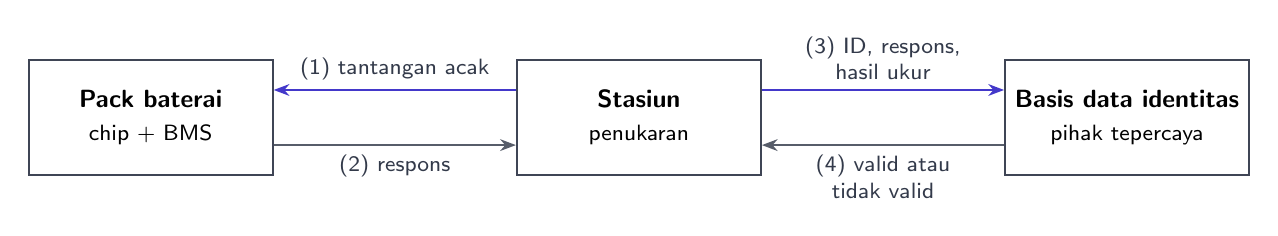
\begin{tikzpicture}[
  font=\sffamily\small,
  actor/.style={draw=ink!80, line width=0.7pt, align=center, minimum width=3.1cm, minimum height=1.45cm, fill=white},
  flow/.style={-{Stealth[length=2mm]}, line width=0.7pt, draw=secline},
  back/.style={-{Stealth[length=2mm]}, line width=0.7pt, draw=ink!70},
  lbl/.style={font=\sffamily\footnotesize, text=ink!85, align=center}
]
  \node[actor] (pack) at (0,0)    {\textbf{\emph{Pack} baterai}\\[1pt]\footnotesize chip + BMS};
  \node[actor] (st)   at (6.2,0)  {\textbf{Stasiun}\\[1pt]\footnotesize penukaran};
  \node[actor] (reg)  at (12.4,0) {\textbf{Basis data identitas}\\[1pt]\footnotesize pihak tepercaya};
  \draw[flow] ([yshift=3.5mm]st.west) -- node[lbl, above]{(1) tantangan acak} ([yshift=3.5mm]pack.east);
  \draw[back] ([yshift=-3.5mm]pack.east) -- node[lbl, below]{(2) respons} ([yshift=-3.5mm]st.west);
  \draw[flow] ([yshift=3.5mm]st.east) -- node[lbl, above]{(3) ID, respons,\\hasil ukur} ([yshift=3.5mm]reg.west);
  \draw[back] ([yshift=-3.5mm]reg.west) -- node[lbl, below]{(4) valid atau\\tidak valid} ([yshift=-3.5mm]st.east);
\end{tikzpicture}
\caption{Alur verifikasi baterai di stasiun penukaran.}
\end{figure}

\section{Poin yang Mohon Ditinjau}

\begin{enumerate}
  \item Ketepatan pembingkaian masalah, terutama penekanan pada baterai yang berpindah lintas operator sebagai alasan perlunya identitas yang dapat diverifikasi secara netral.
  \item Kecukupan data pendukung. Saat ini belum ada data insiden baterai palsu atau kebakaran di jaringan tukar baterai di Indonesia. Apabila Bapak mengetahui sumber yang dapat dirujuk, tim akan sangat terbantu.
  \item Kewajaran klaim terhadap IC autentikasi komersial pada tabel kesenjangan.
\end{enumerate}

\begin{thebibliography}{9}\small
\bibitem{perpres55} Peraturan Presiden RI No.~55 Tahun 2019 tentang Percepatan Program Kendaraan Bermotor Listrik Berbasis Baterai untuk Transportasi Jalan.
\bibitem{perpres79} Peraturan Presiden RI No.~79 Tahun 2023 tentang Perubahan atas Perpres No.~55 Tahun 2019.
\bibitem{ruptl} PT PLN (Persero), \emph{Rencana Usaha Penyediaan Tenaga Listrik (RUPTL) 2025--2034}, hlm.~II-53--II-54.
\bibitem{rukn} Kementerian ESDM, \emph{Rencana Umum Ketenagalistrikan Nasional (RUKN)}, Kepmen ESDM No.~85.K/TL.01/MEM.L/2025, hlm.~51.
\bibitem{eubat} Regulation (EU) 2023/1542 of the European Parliament and of the Council of 12 July 2023 concerning batteries and waste batteries.
\bibitem{barel} H. Bar-El \emph{et al.}, ``The Sorcerer's Apprentice Guide to Fault Attacks,'' \emph{Proceedings of the IEEE}, vol.~94, no.~2, 2006.
\bibitem{suh} G. E. Suh and S. Devadas, ``Physical Unclonable Functions for Device Authentication and Secret Key Generation,'' \emph{Proc. Design Automation Conference (DAC)}, 2007.
\bibitem{maes} R. Maes, \emph{Physically Unclonable Functions: Constructions, Properties and Applications}, Springer, 2013.
\end{thebibliography}

\end{document}
